%%%%%%%%%%%%%%%%%%%%%%%%%%%%%%%%%%%%%%%%%%%%%%%%%%%%%%%%%%%%%%%%%%%%%%%%%%%%%%%%
%2345678901234567890123456789012345678901234567890123456789012345678901234567890
%        1         2         3         4         5         6         7         8

\documentclass[a4paper, 10pt, conference]{IEEEtran}  % Comment this line out if you need a4paper

%\documentclass[a4paper, 10pt, conference]{ieeeconf}      % Use this line for a4 paper

\IEEEoverridecommandlockouts                              % This command is only needed if
                                                          % you want to use the \thanks command


% See the \addtolength command later in the file to balance the column lengths
% on the last page of the document

% The following packages can be found on http:\\www.ctan.org
\usepackage{graphics} % for pdf, bitmapped graphics files
\usepackage{epsfig} % for postscript graphics files
\usepackage{mathptmx} % assumes new font selection scheme installed
\usepackage{times} % assumes new font selection scheme installed
\usepackage[utf8]{inputenc}
\usepackage[onelanguage,ruled,linesnumbered]{algorithm2e}
\usepackage{booktabs} % For formal tables
\usepackage{amsmath}
\usepackage{amssymb}
\usepackage{lipsum}
\usepackage{todonotes}
\usepackage{xcolor}
\usepackage{subfigure}
\usepackage{multirow}

\hyphenation{cen-tra-li-zed}

\newcommand{\packdrop}{$PackDrop$\xspace}
\newcommand{\batchsend}{$BatchSend$\xspace}
\newcommand{\batchassembly}{$BatchAssembly$\xspace}

\newcommand{\distributedlb}{$Distributed$\xspace}
\newcommand{\dummylb}{$Dummy$\xspace}
\newcommand{\greedylb}{$Greedy$\xspace}
\newcommand{\refinelb}{$Refine$\xspace}
\newcommand{\charm}{{\small\texttt{Charm++}}\xspace}

\newcommand\tofix[1]{\textcolor{orange}{#1}}

\title{A Batch Task Migration Approach\\ for Decentralized Global Rescheduling}

% Organizar as linhas de autores de forma diferente. Está muito caótico com múltiplas pessoas da mesma instituição as vezes separadas e as vezes juntas

\author{
\IEEEauthorblockN{Vinicius Freitas$^\star$, Alexandre de L. Santana$^\star$, Márcio Castro$^\star$, Laércio L. Pilla$^{\star\dagger}$\thanks{This work was partially supported by the  Brazilian Federal Agency for the Support and Evaluation of Graduate Education (CAPES) and by the Brazilian Council of Technological and Scientific Development (CNPq), project grant 401266/2016-8.}}
\IEEEauthorblockA{$^\star$ Federal University of Santa Catarina (UFSC), Florianópolis, Brazil\\
$^\dagger$ University of Grenoble Alpes, INRIA, CNRS, Grenoble INP, LIG, France\\
Email: {\smaller\texttt{\{vinicius.mctf,alexandre.santana\}@posgrad.ufsc.br, marcio.castro@ufsc.br, laercio.lima@inria.fr}}}
}

\begin{document}



\maketitle
\thispagestyle{empty}
\pagestyle{empty}


%%%%%%%%%%%%%%%%%%%%%%%%%%%%%%%%%%%%%%%%%%%%%%%%%%%%%%%%%%%%%%%%%%%%%%%%%%%%%%%%
\begin{abstract}

  Effectively mapping tasks of High Performance Computing (HPC) applications on parallel systems is crucial to assure substantial performance gains.
  As platforms and applications grow, load imbalance becomes a priority issue. 
  Even though centralized rescheduling has been a viable solution to mitigate this problem, its efficiency is not able to keep up with the increasing size of shared memory platforms.
  To efficiently solve load imbalance today, and in the years to come, we should prioritize decentralized strategies developed for large scale platforms.
  In this paper, we propose our \textit{Batch Task Migration} approach to improve decentralized global rescheduling, ultimately reducing communication costs and preserving task locality.
  We implemented and evaluated our approach in two different parallel platforms, using both synthetic workloads and a molecular dynamics (MD) benchmark. 
  Our solution was able to achieve speedups of up to 3.75 and 1.15 on rescheduling time, when compared to other centralized and distributed approaches, respectively. 
  Moreover, it improved the execution time of MD by factors up to 1.34 and 1.22 when compared to a scenario without load balancing on two different platforms.

\end{abstract}

\begin{IEEEkeywords}
High Performance Computing, Global Rescheduling, Load Balancing, Performance Evaluation, Parallel Algorithms
\end{IEEEkeywords}

\section{Introduction}

%\begin{itemize}
%	\item Motivation: Why load balancing
%	\item Context: Scenarios in which global rescheduling applies
%	\item Problem: Scaling iterative applications: algorithm limitations
%	\item Justification: Scalable load balancing, distributed rescheduling
%	\item Related work: Hierarchical (limited scaling), Distributed (excessive comm), Diffusive (iterative), Refinement Based (centralized)
%	\item Proposed solution: Batch task migration to mitigate communication costs
%	\item Paper contributions	
%	\item Results brief
%	\item Paper structure
%\end{itemize}

%Growth of systems and applications.
%Need to achieve high scalability to use platforms.
%Efficient scheduling and use of resources.
%
%Dynamic iterative applications.
%Unable to use work stealing.
%Global rescheduling as a solution.
%
%Strong scaling of applications.
%Cost of centralized load balancing.
%Using platform parallelism to achive performance.
%Communication costs as a relevant overhead.
%
%Present hierarchical LB.
%Pros: weak scaling, topology.
%Cons: high comms, bottlenecks.
%Present distributed LB.
%Pros: parallel, refinement.
%Cons: high comms, network contention.
%
%\textbf{Cut out topo aware and diffusive, not related enough.}
%
%Brief intro to BTM.
%Reduced communication.
%Highly parallel.
%Fast convergence.
%
%Present contributions.
%
%Brief results.
%
%Present paper structure.
%
%\hline

Parallel machines are at their best when the workload is evenly distributed among compute nodes, and idle time is merely a myth.
Unfortunately, strong scaling applications for these platforms has been a challenge as long as they have existed.
In this context, uneven workload distribution and high communication overheads are the main villains when developing parallel applications~\cite{Deveci2015}.
Concerns towards these problems increase as systems grow in size and performance, consuming more resources, specially power, to solve some of the most complex problems in scientific computing~\cite{exapower2015,padoin2017energy}.

Applications such as simulations of molecular dynamics (MD) and hydrodynamics suffer from load imbalance due to their intrinsic dynamic and iterative nature~\cite{namd,IPDPS13:LULESH}.
Although rescheduling algorithms have been able to greatly improve the performance of these applications~\cite{namd}, new approaches are needed to guarantee their performance as parallel systems grow.
Since mapping tasks to processing elements (PEs) is an NP-Hard problem~\cite{npcomplete}, the increase in application data and platform size makes centralized rescheduling approaches inefficient.
This creates a need for scalable and decentralized rescheduling approaches, avoiding both excess of data to process and network contention~\cite{trahay2009scalable}.

The two main paths to achieve scalability in global rescheduling for iterative applications are \textit{hierarchical} and \textit{distributed} approaches.
Hierarchical load balancing explores parallelism using different approaches for fine-grain and coarse-grain steps~\cite{hybrid}.
Although scalable, hierarchical schedulers are often tied to the same limitations of centralized approaches, as data is still aggregated in parent nodes.
On the other hand, distributed load balancing approaches seek to achieve scalability through multiple smaller, decentralized scheduling decisions.
Albeit more scalable than hierarchical approaches, decentralized schedulers have limited system information and often incur in higher amounts of communication.

Despite their notable effectiveness, few are the distributed strategies in the domain of global rescheduling~\cite{diffus,grapevine}.
In this paper, we present the concept of \textit{Batch Task Migration} and a novel distributed global rescheduling algorithm that applies this technique, called \packdrop.
Our approach is based on the idea of grouping tasks in batches prior to migration decisions, decreasing the communication overhead in the scheduling decision time and preserving the locality of migrated tasks~\cite{Paudel2013wslocal}.

% Main contributions
In this paper, we present the following contributions: 
\begin{enumerate}
	\item A highly scalable \textit{Batch Task Migration} approach for distributed rescheduling algorithms;
	\item A novel distributed rescheduling algorithm, \packdrop, using our \textit{Batch Task Migration} approach;
	\item An implementation of our algorithm in a well-known parallel programming model as well as a performance evaluation of this implementation.
\end{enumerate}

The remainder of this paper is divided as follows.
Section~\ref{sec:rw} discusses recent work in dynamic rescheduling of scientific applications. 
Section~\ref{sec:algo} presents our novel approach and the developed algorithms. 
Section~\ref{sec:analysis} presents a complexity analysis of our distributed algorithm (\packdrop). 
Section~\ref{sec:impl} displays implementation details, execution environments and benchmarks used in this paper. 
Section~\ref{sec:eval} presents our performance evaluation methodology and discusses the obtained results. 
Finally, Section~\ref{sec:conclusion} presents the conclusion of this work and our plans for future research.



\section{Related Work}

Global rescheduling is a well studied theme in high performance computing~\cite{Deveci2015,grapevine,nuco,hybrid,ZoltanParHypRepart07,diffus,Zheng2010}. 
In the centralized domain, strategies implement a variety of heuristics in order to achieve an homogeneous distribution of load.
Although centralized algorithms are used the most, they lack scalability and new approaches must be pursued as systems grow.

Refinement based solutions in centralized load balancing are very effective in dealing with low imbalance or high migration costs~\cite{MenonPHD}. 
Since these strategies use a limited migration heuristic, they are able to efficiently balance load with a low overhead.
However, since refine strategies limit a total number of migrations, they cannot deal with very unbalanced systems.
\todo[inline]{Citar balanceadores centralizados é mesmo necessário? Não parecem faltar referencias de distribuídos para colocar algo distante como relacionado}

Different approaches have been used to scale scheduling strategies.
Hierarchical algorithms will work differently in different levels, exploring parallelism and delivering better performance~\cite{nuco,hybrid,GengbinThesis}.
Strategies in this domain have been able to ensure scalability so far, but are still limited by a centralized beginning and data dependency.

Also in the hierarchical domain, multilevel graph partitioning has been used to efficiently reschedule tasks~\cite{ZoltanParHypRepart07}.
The hypergraph abstraction accurately represents communication, which provides more precision for load balance~\cite{commaware,Bathele2011graph}.
However, the cost of this representation is very high for a first task mapping process, being more recommended for repartitioning.

Work stealing is one of the most broadly used techniques for balancing load in parallel systems~\cite{DBLP:journals/ijpp/YangH18,Janjic2013}.
The completely distributed essence of this techniques make them very effective scheduling solutions for parallel and distributed irregular applications.

Diffusive load balancing is a completely distributed solution that may benefit iterative applications~\cite{diffus}.
These schedulers irradiate work from overloaded PEs to their neighbors, in an effort to achieve load balance in an iterative fashion.
Very unbalanced systems suffer with this kind of approach, since the scheduler may take too long to reach a solution.

\textit{Grapevine} is a completely distributed refinement-based scheduling solution.
It uses probabilistic transfer of load and epidemic communication protocols to achieve scalability~\cite{grapevine}.
We intend to use what was created in \textit{Grapevine} and reduce its communication, using the \textit{Task Packing} approach.

\todo[inline]{Add related work on BinLPT \@ Marcio}
\todo[inline]{Add related work to MigBSP~\cite{MigPFrighi} \@ Pilla}
\section{Batch Task Migration Approach} \label{sec:algo}

%Global rescheduling algorithms must be effective in order to improve scheduling, but should also have low overhead in order to avoid reducing its benefits.
%To ensure a quick and informed remapping of tasks, we present the \textit{Task Packing Approach}.
%Sharing global information (e.g. processor affinity, estimated computational load, expected communication patterns, etc) allows a PE to create groups of the best tasks to leave a given processor and take the migration decision with one message, instead of several.

%\todo[inline]{Mesmo tendo falado que o algoritmo é distribuido, vale a pena ressaltar que os algoritmos apresentados executam um por PE. Done: Linha 25}

The role of the global rescheduler is to ultimately reduce the application makespan. 
Thus, the scheduler policy must incur low overheads as to not overshadow its benefits. 
Moreover, we envision that a \textit{Batch Task Migration} approach can ensure a quick and informed remapping of tasks, ultimately reducing the amount of messages during the scheduling decision process. 
Therefore, this section is dedicated to present our \packdrop strategy as a distributed refinement-based technique that implements our proposed \textit{Batch Task Migration} approach.

%In this work we present the \textit{PackDrop} strategy, a distributed refinement-based technique implementing our new approach. 
Overall, our approach intends to:

\begin{enumerate}
	\item \textit{Reduce unnecessary communication} between PEs;
	\item \textit{Exploit task locality} within PEs, since migrations are done in groups;
	\item \textit{Accelerate the decision making process}, consequence of the first; and
	\item \textit{Reduce the application makespan}.
\end{enumerate}

We first explain two algorithms that are used by \packdrop: \batchassembly (Algorithm~\ref{alg::packcreation}) and \batchsend (Algorithm~\ref{alg::packsend}).
Then, the complete strategy, called \packdrop, will be presented in Algorithm~\ref{alg::packdrop}.
We assume that the \packdrop algorithm is executed on each PE and communicates with other remote \packdrop instances via message passing.
For clarity, all symbols used in the algorithms are listed in Table~\ref{tab:algo:symbols}.

%\todo[inline]{Qual a lógica para a ordem na tabela? Aceito opiniões sobre como ordenar a tabela}

\begin{table}[t]
	\centering
	\caption{List of symbols, variables and functions.}
	\resizebox{\columnwidth}{!}{
	\begin{tabular}{l l l}
		\toprule
		\textbf{Symbol} & \textbf{Meaning} & \textbf{Definition}\\ 
		\midrule
		$v$				& Load threshold in \% 								& Equation~\ref{eq:ceil} \\
		$ub(load,v)$		& Upper bound of $l$ with threshold $v$		 		& Equation~\ref{eq:ceil} \\
		$load$			& Compute load of the local PE \\
		$load_{task}(t)$	& Compute load of a task $t$							& Equation~\ref{eq:load}	\\
		$load_{set}(T)$	& Load of a set ($T$) 								& Equation~\ref{eq:load} \\
		$T$				& Set of tasks 										& Equations~\ref{eq:load},~\ref{eq:taskmap} \\		
		$M$				& Mapping of tasks									& Equation~\ref{eq:taskmap} \\
		& &\\	

		$\rightarrow$ 	& Remote procedure call 								& Section~\ref{sec:algo} \\
		$\Rightarrow$ 	& Reduction process 									& Section~\ref{sec:algo} \\
		$load_{avg}$		& Average system load of a PE 						& Section~\ref{sec:algo:creation}\\ 
		$s$			  	& Compute load in a batch of tasks 					& Section~\ref{sec:algo:creation} \\
		$rand(S)$		& Random element of $S$ 								& Section~\ref{sec:algo:sending} \\
		$P$				& Global set of PEs 									& Section~\ref{sec:algo:main} \\
		$Gossip$			& Start of information propagation					& Section~\ref{sec:algo:main} \\		
		$pack$			& Set of leaving tasks								& Section~\ref{sec:algo:main} \\
		& &\\
				
		$LT$				& Set of tasks leaving a PE 							& Algorithm~\ref{alg::packcreation} \\
		$L$				& Set of tasks, subset of $LT$						& Algorithm~\ref{alg::packcreation} \\
		$G$				& Target for task receiving							& Algorithm~\ref{alg::packsend} \\
		$BG$				& Pairs expecting migration ack						& Algorithm~\ref{alg::packsend} \\ 
		$Send(T)\rightarrow G $ & Send a set $T$ to target $G$				& Algorithm~\ref{alg::packsend} \\ 
		$Id_l$ 			& Local PE identifier								& Algorithm~\ref{alg::packdrop} \\
		$TaskMap$		& Call runtime system to start migrations					& Algorithm~\ref{alg::packdrop} \\
		\bottomrule
	\end{tabular}
	}
	\label{tab:algo:symbols}
\end{table}

\subsection{\batchassembly Algorithm} \label{sec:algo:creation}

The \batchassembly algorithm is presented in Algorithm~\ref{alg::packcreation}.
It uses an estimated batch size ($s$), a set of local tasks ($T$), the current PE $load$ and a threshold for PE loads ($v$), to create a set of leaving tasks ($LT$).
The threshold is used to calculate an upper bound of the average system load ($load_{avg}$), using Equation~\ref{eq:ceil}. 
The load of any set of tasks is given by Equation~\ref{eq:load}.

\begin{equation}
	ub(load,v) = (1+v)\times load
    \label{eq:ceil}
\end{equation}
\begin{equation}
	load_{set}(T) = \sum_{t \in T}{load_{task}(t)}\ \ |\ \ T \text{ is a set of tasks}
	\label{eq:load}
\end{equation}

With this information, each PE will take the task with the smallest load within its pool, and add it to a set of tasks ($L$) (lines~$3-5$).
Then, if the sum of all tasks in the pack is greater than the expected batch size ($s$), the batch is assembled and the strategy starts creating another one (lines~$6-9$).
The process is repeated until the load of the set becomes greater than the upper bound~(line~$2$).

Any unfinished $LT$s should be sent even if those are not complete.
This is done to avoid having an overloaded PE that can still migrate tasks.
A PE that receives this load will not receive as much load as others, but since the PE will not overload, it should not be prejudicial to global system balance.

\begin{algorithm}[b]
    \DontPrintSemicolon
    \KwIn{$s$, expected load of a batch; $T$, set of local tasks; $load_{avg}$, average global PE load; $v$, imbalance tolerance ratio.}
    \KwOut{$LT$, set of tasks leaving this PE.}
    $L \gets \varnothing,\ LT \gets \varnothing$ \\
    \While{$load_{set}(T) > ub(load_{avg},v)$}{
        $t \gets a \in   T\ |\ a$ is the lower bound of $T$\\
        $  T \gets   T\ \backslash\ \{t\} $\\
        $\textit{L} \gets L\ \cup\ \{t\}$\\
        %$load \gets load - t$\\
        \If{$load_{set}(L) > s$}{
            $LT \gets LT\ \cup\ L$\\
            $L \gets \varnothing $
        }
    }
    $LT \gets LT\ \cup\ L$   
    \caption{\batchassembly} 
    \label{alg::packcreation}
\end{algorithm}

\subsection{\batchsend Algorithm} \label{sec:algo:sending}

The \batchsend algorithm is presented in Algorithm~\ref{alg::packsend}.
The algorithm will use the $LT$s, produced by \batchassembly, and the set of $Targets$, produced by an information propagation step ($Gossip$~\cite{gossip}), in order to schedule packs on remote PEs.
This will produce a set of expected Batch/Target ($BG$) pairs, which should be confirmed by the remote target.

For each subset $b \subset LT$ (as assigned in Algorithm~\ref{alg::packcreation}), the algorithm will select a random target from $G$~(line~$3$).
It will invoke a remote $Send$ procedure on the target $g$~(line~$4$), and register its attempt in a pair ($b$, $g$).
This pair is then stored in the expecting confirmation set ($BG$) (line~$5$).

\begin{algorithm}[t]
    \DontPrintSemicolon
    \KwIn{$LT$, set of tasks leaving the local PE; $G$, set of possible migration targets.}
    \KwOut{$BG$, set of expected migrations.}
    $BG \gets \varnothing$ \\
    \ForEach{$b \subset LT$}{
        %$b\ \gets p\ |\ p\ \in\ LT$\\
        $g\ \gets  rand(G)$\\
        $Send(b)\rightarrow g$\\
        %$LT\ \gets\ LT\ \backslash\ \{b\}$\\
        $\textit{BG} \gets BG\ \cup\ \{(b,\ g)\}$\\
    }  
    \caption{\batchsend}  
    \label{alg::packsend}
\end{algorithm}

In case of negative responses from remote $Send$ procedures, Algorithm~\ref{alg::packsend} may initiate another round of sends with the failed attempts so every member of $LT$ is migrated.

\subsection{\packdrop Algorithm} \label{sec:algo:main}

The \packdrop strategy is presented in Algorithm~\ref{alg::packdrop}.
For simplicity, in the explanation of this algorithm \textit{packs} will be a short for ``set of leaving tasks" (seen in Sections~\ref{sec:algo:creation}~and~\ref{sec:algo:sending}).

\packdrop will run individually on each PE, in a distributed fashion. 
It will produce a new mapping ($M'$) using a current local mapping of tasks to PEs ($M$), local load ($load$), a local PE identification ($Id_l$) and the global set of PEs ($P$).
The mapping of tasks is defined by Equation~\ref{eq:taskmap} as a set of pairs ($task, PE$), which describe the location of tasks.
A local mapping of tasks contains only tasks that are assigned to the current PE.

\begin{equation}
	M:\ T \rightarrow P
	\label{eq:taskmap}
\end{equation}

The first part of the algorithm (lines $1-6$) is the information sharing and setup process. 
This process is done through $2$ global reductions of average PE load (line~$2$) and global number of tasks (line~$3$).
\tofix{
	In this implementation we used two constants. The first one ($v$) was set to $0.05$ in order to limit the imbalance at $5\%$ (line~$5$).
	The second one was defined in $ps$ and set to $2$ in order to regulate the size of packs (line~$6$).
	The value of $ps$ is defined by Equation~\ref{eq:ps}. The rationale behind this is... COMPLETE THE SENTENCE.
}

\begin{equation}
	ps = 2-\frac{|P|}{ttc}
	\label{eq:ps}
\end{equation}

Next, PEs are divided between two different workflows (line~$7$).
At this time, \textit{overloaded} PEs will start the \batchassembly algorithm (line~$8$), which was previously explained in Algorithm~\ref{alg::packcreation}.
Meanwhile, \textit{underloaded} PEs will initiate a \textit{Gossip Protocol}~\cite{gossip} in order to inform other elements they are willing to receive work (line~$11$).
\textit{Gossip} is a well-known epidemic algorithm used to spread messages on a system, providing fast convergence and near-global awareness of shared information.

Once information propagation is done, each PE must synchronize to start the remapping process (line~$13$). 
At this point, PEs will send their packs using \batchsend (Algorithm~\ref{alg::packsend}) asynchronously (line~$14$).
After a pack is sent, PEs will accept or reject it based on their current load, this is done via \textit{three-way handshake}, so both parts confirm the migration.

\begin{algorithm}[t]
	\DontPrintSemicolon
    \KwIn{$M$, local mapping of tasks; $load$, local PE load; $P$, set of all PEs in the system; $Id_{l}$, local PE identifier.}
    \KwOut{$  M'$, new mapping of local tasks.}
    $  M' \gets \varnothing$\\
    $load_{avg} \gets (AveragePeLoadReduction(load)\Rightarrow  P)$ \\
    $ttc \gets (TotalTaskCountReduction(|M|)\Rightarrow  P)$\\
    $ats\gets \frac{load_{avg}}{ttc}$ \qquad\qquad\qquad \tcp{{\small Average~task~size}}
    $v \gets 0.05$ \qquad \qquad\ \tcp{{\small 5\%~precision~on~balance}}
    $s \gets ats\times ps$ \qquad\qquad\qquad\qquad\qquad \tcp{{\small Pack load}}
    \uIf{$load > ub(load_{avg},v)$}{
    	$packs \gets BatchAssembly(s,  T(M),load,v)$
    }
    \Else{
    	$packs \gets \varnothing$\\
    	$G \gets (Gossip \rightarrow  P)$ \tcp{{\small Targets for migration}}
    }
    $---Synchronization Barrier---$\\
    \tcc{{\small Requests are processed as they are received back}}
    $R \gets BatchSend(packs, G)$\\
    \tcp{{\small Implicit synchronization in TaskMap}}
    $TaskMap(R,M, M',Id_{l})$
    \caption{\packdrop}
    \label{alg::packdrop}    
\end{algorithm}

If one or more packs were not successfully exchanged, an \textit{overloaded} PE must attempt a new \batchsend, in order to achieve load balance, as specified in Section~\ref{sec:algo:sending}.
Once the PEs know their new mappings, tasks are migrated and the strategy is finished, requesting the confirmed migrations to the RTS (line~$15$). 
The $TaskMap$ function will take care of informing the new mapping ($M'$) to all tasks received via $Send$ and removed via \batchsend.

\packdrop intends to remap tasks to PEs in a distributed, workload-aware fashion.
This approach is the basis for new batch task migration distributed strategies that may take other factors into account.


\section{Analysis of the Algorithm} \label{sec:analysis}

This section presents an analysis of \packdrop (Algorithm~\ref{alg::packdrop}). 
Symbols presented in this section are available on Tables~\ref{tab:algo:symbols}~and~\ref{tab:analysis:symbols}.
The complexity of the information propagation ($Gossip$) has being evaluated as $O(log_{fout}n)$~\cite{grapevine},
where $fout$ is the $Gossip$ fanout and $n$ is the number of PEs in the system.
Here we use $fout=2$, in order to avoid network congestion. 

For the sake of simplicity, in the remainder of this analysis, the number of tasks in the system
will be referred to as $m$, and the costs for computation and communication will be represented as $p_c$ and $c_c$, respectively.
We also assume $c_c > p_c$ for all concurrent scenarios, since communication costs are several orders of magnitude higher than computational costs.
$C(A)$ is referred here as the complexity class of a given workload $A$, similar to its total cost.
Unmentioned lines are assumed to have non-varying costs, and thus will not interfere in the asymptotic analysis.

Lines~2~and~3 are global reductions, which have a well-known cost of $O(log\ n)$.
Lines~8~and~11 are concurrent, so their cost will be the maximum among them:
\begin{equation}
  max(C(BatchAssembly),C(Gossip))
\end{equation}

We also know that the worst case for \batchassembly (Algorithm~\ref{alg::packcreation}) is rather unrealistic, 
since it would assume that a single PE contains $m$ tasks and a single task may have a load greater than the average system load, being $O(m-1)$, assuming $1$ would not be migrated, asymptotically, $O(m)$.

\begin{table}[t]
	\caption{List of symbols used in the Analysis of the Algorithm.}
	\centering	
	\begin{tabular}{l l}
		\toprule
		\textbf{Symbol}		& \textbf{Meaning} \\
		\midrule
		$fout$			& $Gossip$ protocol's \textit{fanout} \\ 
		$p_c$			& Computational (processing) base cost \\
		$c_c$			& Communication base cost \\
		$C(A)$			& The complexity class of a given function $A$ \\
		$m$				& Number of tasks in the system \\
		$m_l$			& $max(|T|)$ in an overloaded PE \\
		\bottomrule
	\end{tabular}
	\label{tab:analysis:symbols}
\end{table}

Thus, the cost of lines~8~and~11 is:
\begin{equation}
 max((p_c\times m),\ (c_c\times log\ n))
\end{equation}
and since $c_c$ is several orders of magnitude bigger than $p_c$, we could assume $C(BatchAssembly) \in C(Gossip)$, which makes the 
complexity of these lines to $O(log\ n)$.

Finally, line~14 will have a complexity equal to the largest number of packs migrated by an overloaded PE.
Let $ps$ be the average number of tasks inside of an $LT$, and $m_l$ the maximum number of tasks in a given overloaded PE.
At this step, a solution without \textit{Batch Task Migration} would have a cost of $c_c\times m_l$, while our approach will divide this complexity by $ps$. 
This is the most expensive part of Algorithm~\ref{alg::packdrop}, and as such it is the most interesting one to optimize.
Our final asymptotic complexity is:

\begin{equation}
 C(PackDrop) = O(m_l/ps) + O(log\ n)
 \label{eq:worstcase}
\end{equation}

This shows that determining a good $ps$ value is crucial to achieve the best performance with this algorithm.
Higher values of $ps$ will lower communication complexity, but may lead to an imprecise scheduling.
In our implementation, we chose to vary the value of $ps$ around a base value of $2$, according to system load and characteristics, as described in Equation~\ref{eq:ps}.
\batchassembly (Algorithm~\ref{alg::packcreation}) stores tasks in $LT$ in an increasing load order.
So, even though our average pack should have around $2$ tasks, as their load vary, we are able to include more tasks at a lower communication cost.
This way, we attempt precise load balance, while still preserving task locality after migration.

It is important to note that different applications may react differently to different values of $ps$.
This is specially related to application load variance.
The $ps$ factor may be fine-tuned to each specific application and platform, but we believe a reasonable, generic, approach such as the provided by Equation~\ref{eq:ps} is enough to provide balance to most applications and systems, while still harvesting the advantages of the \textit{Batch Task Migration} approach.

\section{Implementation}

\textit{PackDrop} was implemented as a load balancing strategy in \texttt{Charm++}\footnote{Available at: \texttt{https://github.com/OMMITED-FOR-BLIND-REVIEW}}.
\texttt{Charm++} is a parallel programming model that provides a \textit{load balancing framework} based on migration of its parallel, message-driven objects, the \textit{chares}~\cite{CharmLOTR}.
\textit{Chares} are mapped as \textit{tasks} onto PEs and the \texttt{Charm++} runtime system (RTS) provides the load information needed for the \textit{PackDrop} strategy.

The \texttt{Charm++} RTS allows for the desired asynchronous behavior of \textit{PackDrop}.
It also provides necessary reduction and quiescence detection mechanisms, used in this implementation.
Reductions are used to evaluate the total number of chares and the average load in the system, while the quiescence detection is necessary to finalize the information propagation step of the algorithm.

\texttt{Charm++} provides application-independent load balancing, which means that any application (that implements a PUP framework~\cite{sc14charm}), may use global rescheduling strategies implemented for this RTS.
This means that any of the available applications for \texttt{Charm++} can be used to evaluate our strategy and compare it to other load balancers available for this RTS.


\subsection{Benchmarks} \label{sec:benchmarks}

We experimented our strategy with $2$ benchmarks that are publicly available for \texttt{Charm++}.
The first is a synthetic benchmark called \textbf{LB Test}. 
It simulates work with a variety of communication topologies, such as ring, meshes and randomized patterns.
\textit{LB Test} is known to have a low migration cost, with light \textit{tasks}, and most of its load bound to computation, instead of communication.

The second is a molecular dynamics (MD) mini-app called \textit{LeanMD}\footnote{Available at: \texttt{http://charmplusplus.org/miniApps}}.
This mini-app simulates the behavior of atoms and it mimics the force computation done in the state-or-the-art MD application NAMD, winner of the Golden Bell Award~\cite{grapevine}.
LeanMD uses geometric decomposition in a three-dimensional ($3$D) simulation space.
However, since the number of simulated atoms in each region affects the number of exchanged messages, it has an irregular and dynamic communication pattern, even though it respects the geometric distribution.

\subsection{Other schedulers}

\textit{PackDrop} was compared strategies available on the \texttt{Charm++} benchmark suite.
More specifically, strategies that may be selected by \texttt{Charm++}'s workload-aware \textit{Meta-balancer}~\cite{MenonPHD}.
Their behavior is briefly presented ahead.

\begin{itemize}
	\item \textit{Refine} is a refinement-based strategy that tries to minimize the number of migrated \textit{tasks}, exchanging load among PEs.
This strategy is specially efficient if the imbalance isn't too high.
	\item \textit{Greedy} creates two heaps, one for \textit{tasks} (max-min) and one for PEs (min-max). 
Then, it assigns tasks to PEs, putting the most work-heavy tasks on the least loaded PEs.
This strategy provides a good load balance, but may incur in high migration overhead.
    \item \textit{Distributed}, also known as \textit{Grapevine}, is a distributed strategy based on epidemic communication and probabilistic transfer of work.
   This strategy has good scalability, but does not performs as well as centralized ones in smaller scenarios.

\end{itemize}




\section{Performance Evaluation}

Two platforms were for performance evaluation of our novel \textit{PackDrop} scheduler:
i) A tightly coupled \textit{Supercomputer} with $24$ (in $2$ separate NUMA nodes) PEs per node, using an Infiniband interconnection supported by Intel's Parallel Studio XE implementation of \texttt{MPI} (v2017.4).
ii) A smaller \textit{Cluster} with $4$ PEs per node, using a Gigabit Ethernet interconnection.
Details of both platforms are available on Table~\ref{tab:ptinfo}.

\begin{table}[ht]
    \centering
    \caption{Platform Information of each Node from Supercomputer and Cluster evaluations.}
	\begin{tabular}{c|c|c}
	Node Info.	 		& Supercomputer 		& Cluster \\ \hline
        CPUs	   			& $2\times12$ 			& $4$ \\
        Intel Xeon			& E5-2695v2 			& X3440\\
        CPU Freq.  			& $2.4$GHz   			& $2.53$GHz\\
        RAM        			& $64$GB			& $16$GB\\
        Network 			& Infiniband FDR 		& Gigabit Ethernet\\
        OS      			& RedHat Linux 6.4 		& Ubuntu 14.04\\
        \texttt{GCC}			& $5.3.1$			& $5.4.0$\\
        \texttt{Charm++} 		& $6.8.1$ 			& $6.8.1$\\
        \texttt{MPI}			& $3.1.0$			& -\\
        \texttt{GCC} Flags		& \texttt{-std=c++11 -O3} 	& \texttt{-std=c++11 -O3} \\
	\end{tabular}
    \label{tab:ptinfo}
\end{table}

Ahead we'll present the metrics used to compare our new global rescheduling strategy with \textit{Greedy}, \textit{Refine} and \textit{Distributed}.
Then, we'll discuss results obtained in both platforms descripted in Table~\ref{tab:ptinfo} and the scalability of our proposed solution.
All raw data of our results, as well as parsing scripts for analysis are publicly available\footnote{Available at: \texttt{https://github.com/OMMITED-FOR-BLIND-REVIEW}.}.

\subsubsection*{Metrics}

\textit{Application time} is one of the most relevant metrics to evaluate load balancers in \texttt{Charm++}.
Since migrations may induce high overhead and impact communication costs, a bad algorithm may finish fast, but increase imbalance, and thus, application time.

\textit{Load balancer decision time}, although not the most relevant for the application itself, the decision time is an indicator of its scalability.
Some centralized schedulers, such as \textit{Greedy}, work very well on local machines, with a reasonable data input.
However, when executing on distributed memory environments, the scalability of centralized strategies is limited.

\subsection{Evaluation on Cluster}

All experiments executed on cluster were compiled with \texttt{Charm++} using the \texttt{--with-production} option, combined with the specifications detailed on Table~\ref{tab:ptinfo}.
$32$ homogeneous compute nodes were used, with a total of $128$ PEs.
In addition to previously mentioned schedulers, \textit{Dummy} was added as the representative of a situation with no remap of tasks, it only aggregates the information a centralized strategy needs (its cost is the base for every centralized strategy).

\subsubsection*{Evaluation with Synthetic Load}

\textit{LB Test} experiments had a total of $18990$ \textit{tasks}, executed over $150$ iterations, performing load balance every $40$ iterations.
\textit{Task} loads vary from $30$ms to $9000$ms, which provides reasonable imbalance of load, causing global rescheduling to be useful in this case.
Ring, 2D mesh and 3D mesh communication topologies were used to provide different levels of migration impact and communication cost.

\begin{table}[t]
	\centering
    \caption{LB Test mean application time on the cluster execution.}
	\begin{tabular}{l | c  c  c}
    	Scheduler & Time (Ring) & Time (2D) & Time (3D) \\ \hline
        Distributed & $47.49298$s & $48.64839$s & $49.05481$s \\
        Greedy & $46.54101$s & $49.56052$s & $51.06850$s \\
        Dummy & $52.43016$s & $53.17254$s & $53.94068$s \\
        PackDrop & $46.81598$s & $47.37120$s & $47.97426$s \\
        Refine & $45.49095$s & $46.29277$s & $47.21924$s \\		
	\end{tabular}
    \label{tab:lbtest:apptime}
\end{table}

\begin{figure}
	\centering
    \hspace{-10pt}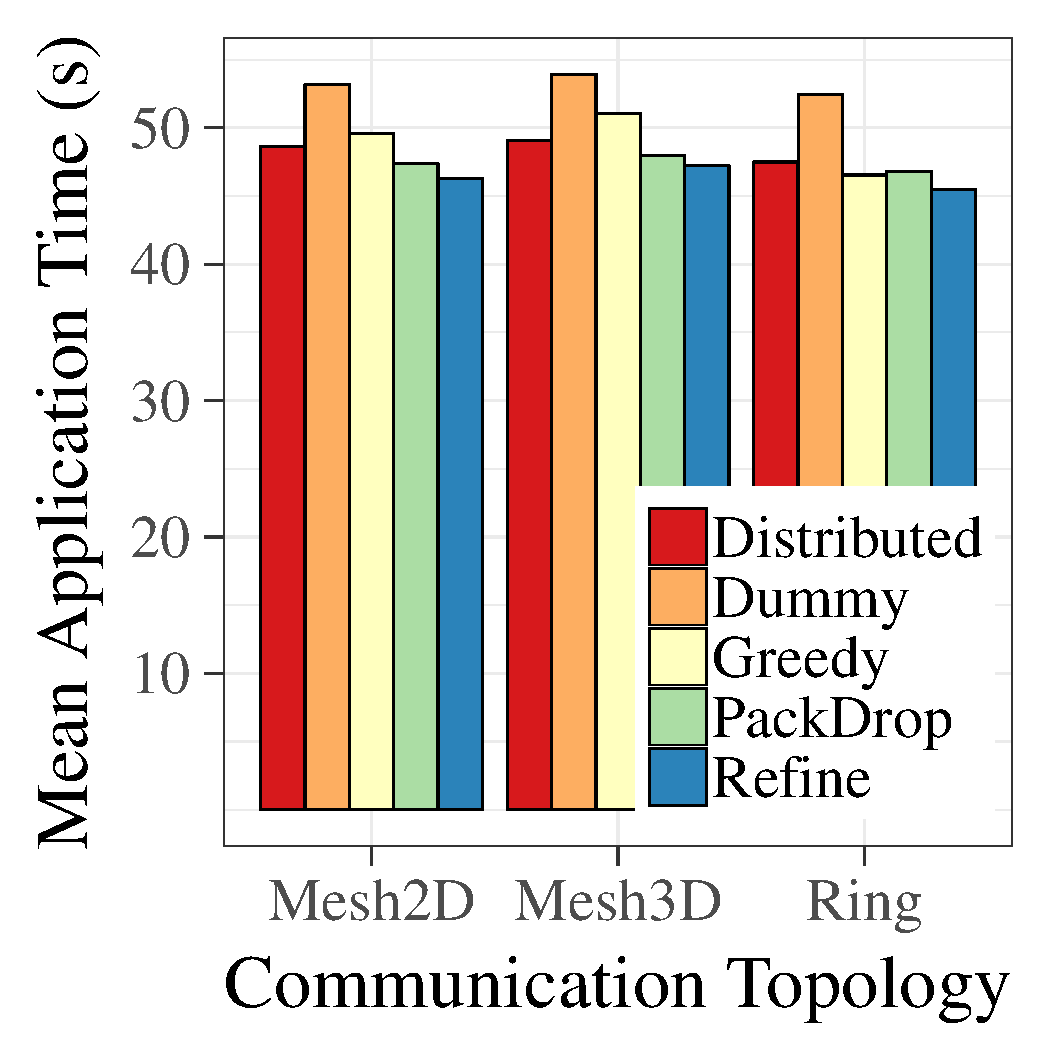
\includegraphics[width=0.5\textwidth]{images/apptime_lbtest_g5k.pdf}
    \caption{LB Test cluster execution results.}
    \label{fig:eval:g5k:lbtest:apptime}
\end{figure}


Each configuration of the benchmark was executed $15$ times, with results depicted on Figure~\ref{fig:eval:g5k:lbtest:apptime} and Table~\ref{tab:lbtest:apptime}.
Results for \textit{Greedy} show how different communication topologies affect the scheduling performance.
Since \textit{Greedy} migrates many \textit{tasks}, the more they communicate, the more migrations impact the application time.

The increased in communication cost can be verified among all scheduling strategies, but in none as much as in \textit{Greedy}.
Our novel approach, \textit{PackDrop} has outperformed the other descentralized strategy, \textit{Distributed}, in the \textit{LB Test} case in this scale.
However, since the platform is not large enough to present all of the potential gains of decentralized strategies, \textit{Refine}, with a reduced migration count approach, still outperforms any other scheduler in this benchmark.
Nevertheless, this indicates a good scalability pontetial, specially in a cluster with high communication overhead, due to its Gigabit Ethernet connection.

\subsubsection*{Evaluation with Molecular Dynamics}

\textit{LeanMD} experiments generated a $9\times9\times9$ space, with a total of $27702$ \textit{tasks}.
Each execution ran $500$ iterations, with a first rescheduling step at the $10$th iteration. 
Rescheduling periods (RP) of every $30$ (short) and every $60$ (long) iterations were used, providing different impacts of rescheduling on the application.
\textit{Greedy} and \textit{Dummy} were excluded from this evaluation due to their high cost in an application such as \textit{LeanMD}. 

\begin{table}[!ht]
	\centering
	\caption{LeanMD mean application time on the cluster execution.}	
	\begin{tabular}{l|c c c}
	Scheduler & Time (Short RP) & Time (Long RP) & Mean LB Time \\ \hline
	Distributed & $69.35606$s & $68.36055$s & $167.0444$ms \\ 
	PackDrop & $55.98428$s & $55.51554$s & $143.1028$ms \\ 
	Refine & $59.35696$s & $55.89895$s & $539.8364$ms \\ 
	\end{tabular}
	\label{tab:eval:g5k:leanmd:time} 
\end{table}

\begin{figure}[!ht]
	\centering
    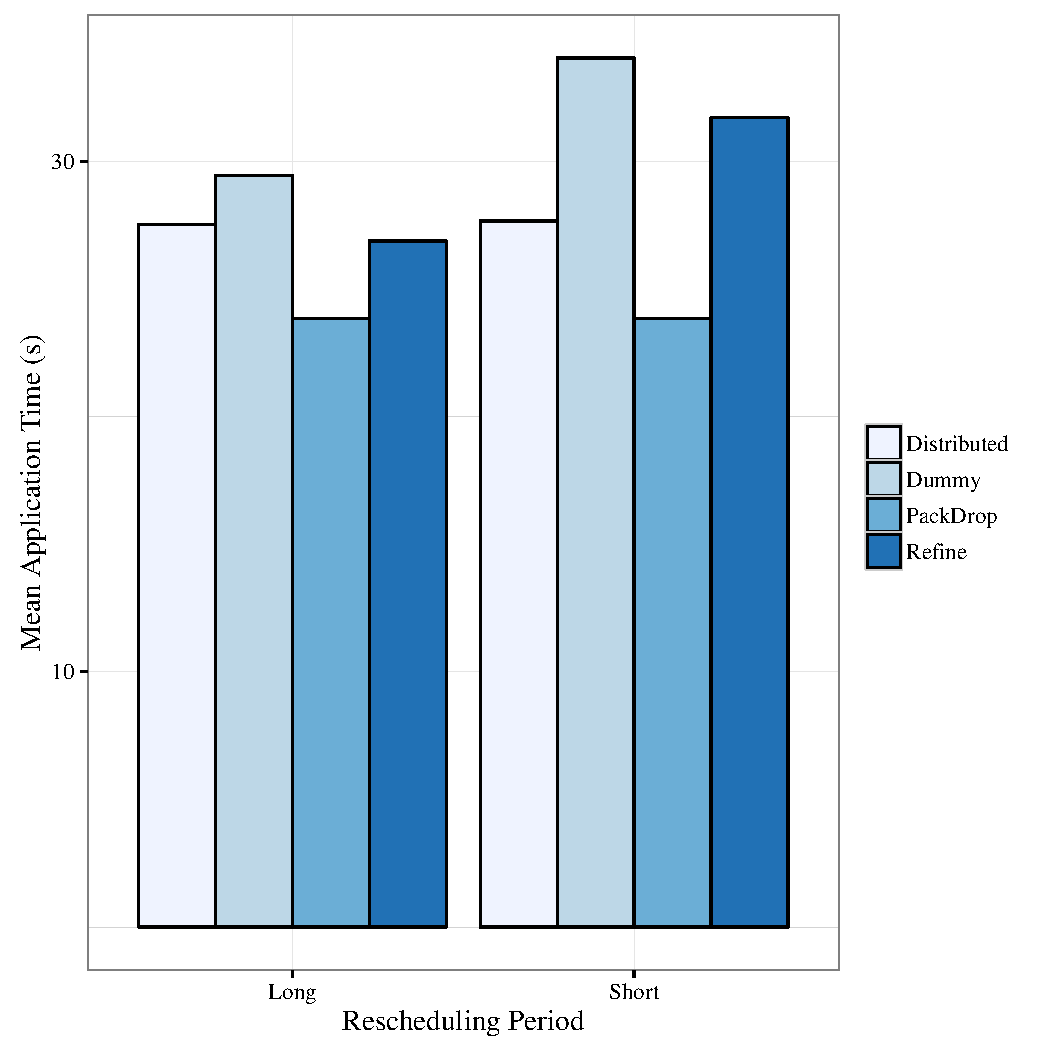
\includegraphics[width=0.43\textwidth]{images/apptime_leanmd_g5k.pdf}
	\caption{LeanMD cluster execution results.}
    \label{fig:eval:g5k:leanmd:time}
\end{figure}

\begin{figure}[!ht]
	\centering
    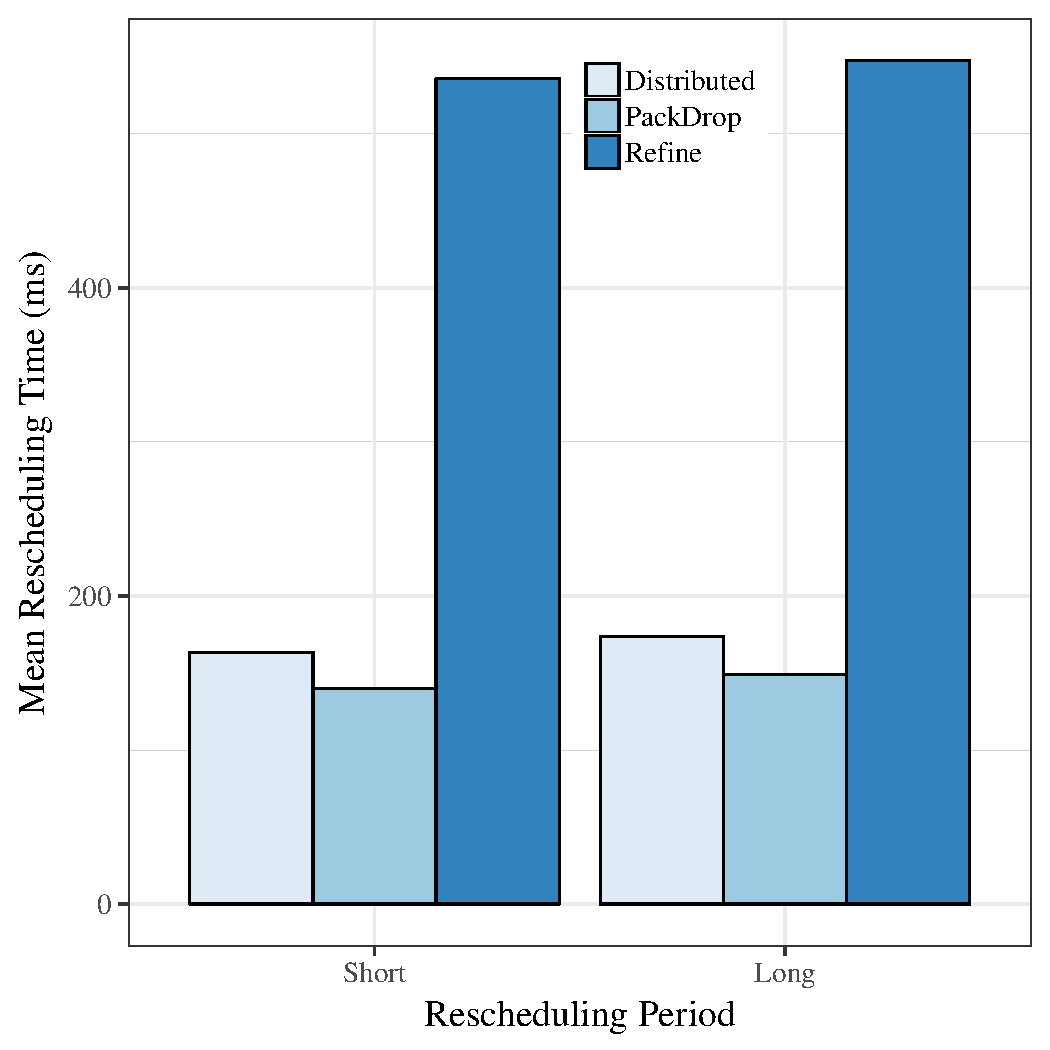
\includegraphics[width=0.43\textwidth]{images/schedtime_leanmd_g5k.pdf}
	\caption{LeanMD cluster execution results.}
    \label{fig:eval:g5k:leanmd:schedtime}
\end{figure}

Each configuration of LeanMD was executed $10$ times, making a total of $5000$ steps per configuration and are depicted in Table~\ref{tab:eval:g5k:leanmd:time} and in Figures~\ref{fig:eval:g5k:leanmd:time},~\ref{fig:eval:g5k:leanmd:schedtime} .
Observed application times presented a standard deviation from the mean lower than $2\%$ for all results presented.

Results show a better overall performance of \textit{PackDrop}, outperforming both compared strategies in the two scenarios chosen.
Since our strategy migrates groups of tasks, it improves locality of tasks after migration, outperforming \textit{Distributed} due to this.

Figure~\ref{fig:eval:g5k:leanmd:schedtime} shows the time taken by the periodical rescheduling (LB), task migration and the first iteration after the LB call.
It shows the increased cost of \textit{Refine}, which is due to both information agregation costs and dealing with the high amounts of application data in a centralized fashion.
\textit{PackDrop} displays its effectiviness in rescheduling time, outperforming both compared strategies, and resulting in an overall better application time. 

\subsection{Evaluation on Supercomputer}

All experiments executed on supercomputer were compiled with \texttt{Charm++} using the \texttt{--with-production} option, combined with the specifications detailed on Table~\ref{tab:ptinfo}.
Different numbers of homogeneous $2\times 12$ PEs compute nodes ($2$ NUMA-nodes with $12$ cores each) were used to evaluate our strategy's scalability.
We ranged from $16$ ($384$ PEs) to $32$ ($768$ PEs) unique nodes in our evaluation. 

\subsubsection*{Evaluation with Molecular Dynamics}

\textbf{LeanMD} experiments generated a $10\times15\times10$ space, with a total of $171$K \textit{tasks}.
Each execution ran $100$ iterations, with a first rescheduling step at the $9$th iteration. 
Rescheduling was performed every $30$ iterations and each configuration of LeanMD was executed $10$ times, making a total of $1000$ steps per configuration. 

\begin{figure}[!ht]
 \centering
 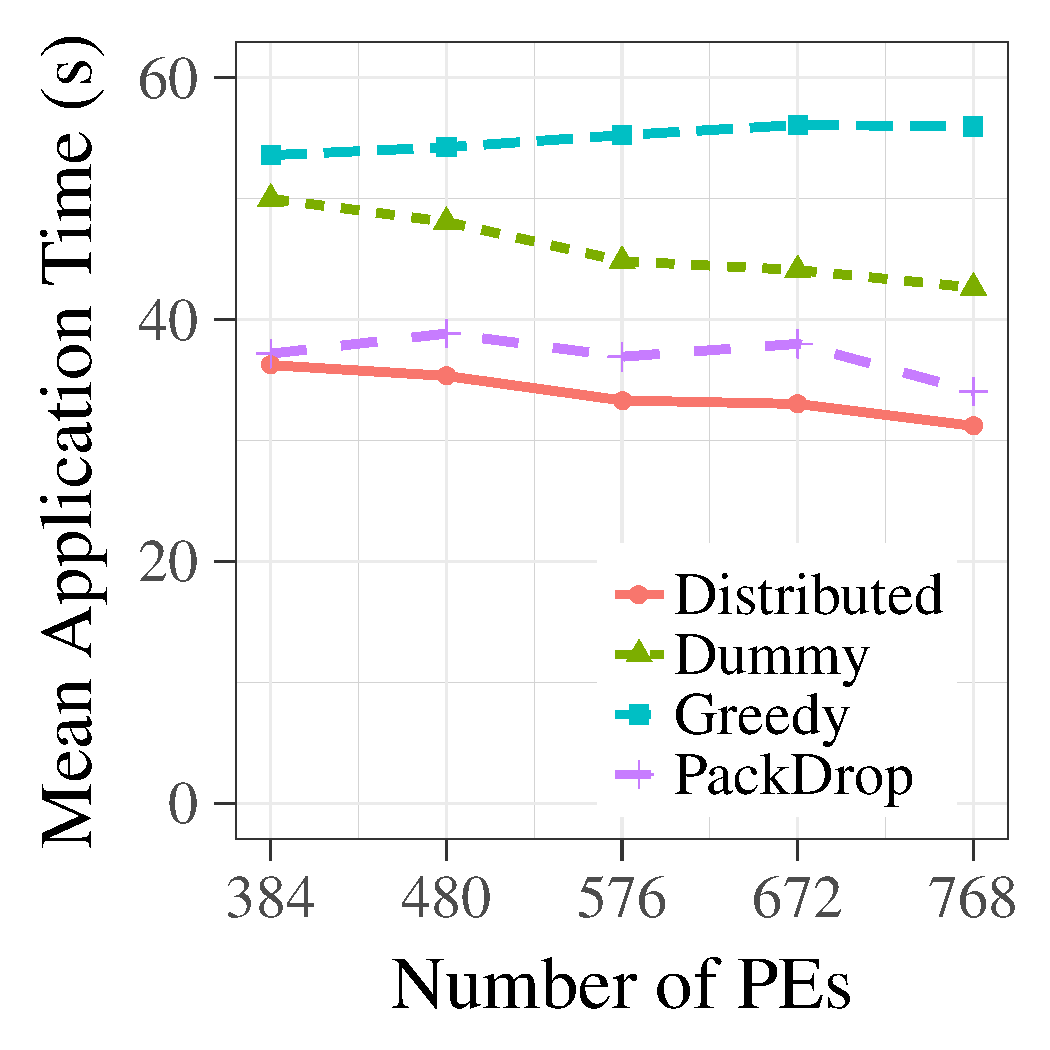
\includegraphics[width=0.9\linewidth]{images/apptime_leanmd_sdumont.pdf}
 \caption{LeanMD supercomputer AppTime execution results.}
 \label{fig:eval:sdumont:leanmd:apptime}
\end{figure}


\begin{figure}
	\centering
	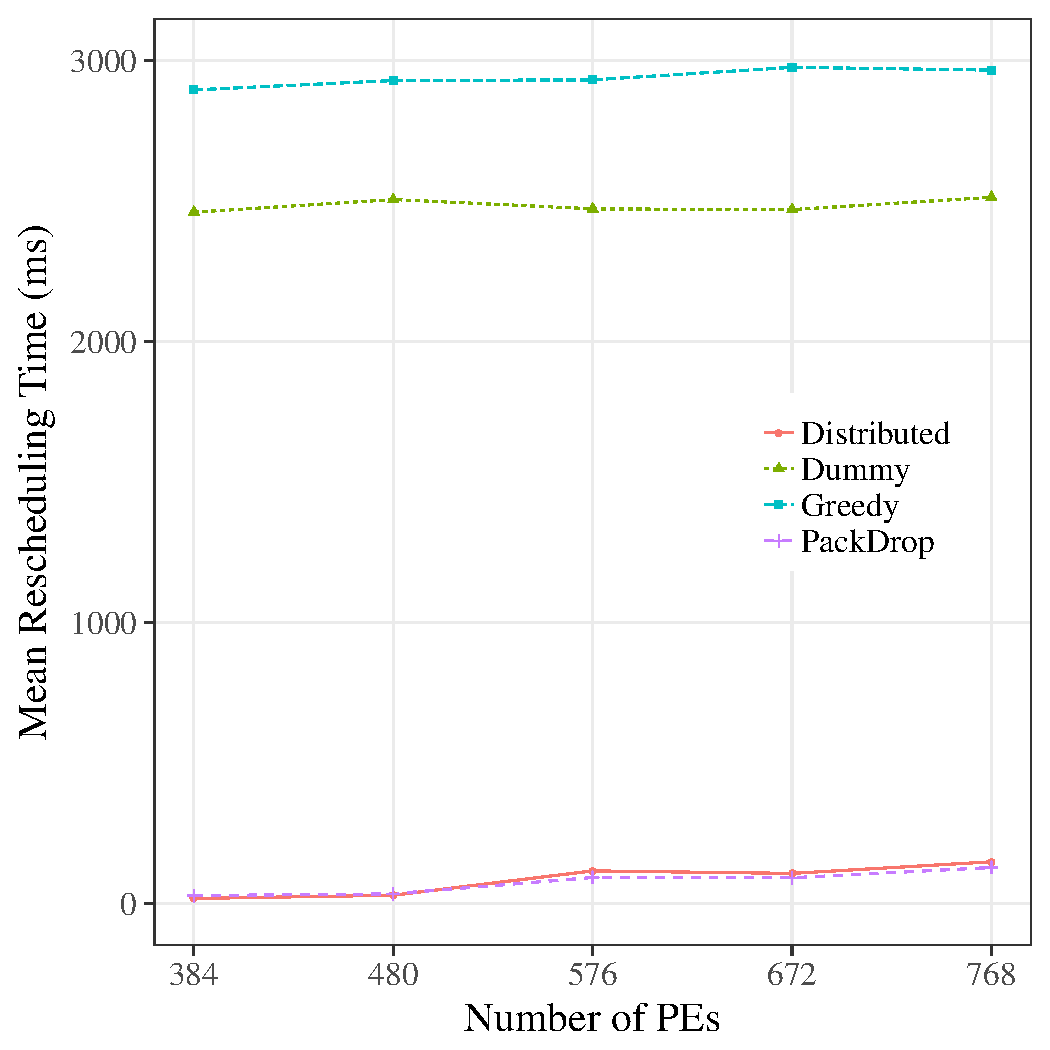
\includegraphics[width=0.9\linewidth]{images/schedtime_leanmd_sdumont.pdf}
	\caption{LeanMD supercomputer SchedTime execution results.}
	\label{fig:eval:sdumont:leanmd:schedtime}
\end{figure}


\subsection{Scalability}
\section{Conclusion} \label{sec:conclusion}

In this paper we have presented the \textit{Batch Task Migration} approach for distributed global rescheduling.
It intends to preserve task communication locality, migrating multiple work units from a source to the same destination, in order to balance system load.
This preserves communication efficiency, while other workload-aware strategies perform rescheduling without considering task locality.

Our approach also mitigates communication costs during algorithm execution time.
We guarantee this by transmitting information about multiple migrations at a time, in \textit{Batches}.
Thanks to this, our novel scheduler (presented in Section~\ref{sec:algo:main}) has an increased performance in high communication overhead platforms, discussed in Section~\ref{sec:cluster}.

We have evaluated our strategy in two different execution environments. 
The first was a high communication cost, $4$ cores/node cluster, executing over $32$ cores.
In this scenario, \textit{PackDrop} had a rescheduling speedup of up to $3.77$ and $1.16$ when compared to centralized and distributed approaches, respectively (Section~\ref{sec:cluster}).

The second scenario was a highly coupled cluster with low communication overhead, with $24$ cores/node.
We executed our experiments varying platform size from $16$ to $32$ nodes.
In this scenario, rescheduling time of \textit{PackDrop} and \textit{Distributed} were very similar, although both had a time up to $3$ orders of magnitude faster than any centralized approach. %Add some data to reinforce this
This reinforces the relevance of work in the distributed scheduling domain, and approaches such as our \textit{Batch Task Migration}.

\subsection{Future Work}

Future work on this theme includes the use of \textit{Batch Task Migration} in the communication-aware domain.
Since our approach already has locality-based benefits, combining this with communication pattern information may incur on even greater performance increase in applications.
We believe a novel strategy focused on the \textit{Stencil} programming model is something to be considered, prioritizing migration of edges among PEs, instead of random parts of the stencil~\cite{stenciltiling}.

Further work will also be developed in order to increase performance in heterogeneous clusters.
These may have heterogeneous processing capacities and network capabilities, which enhances complexity of load balancing significantly.
In this given scenario, enhancing rescheduling decision processes may be crucial to ensure gains in application performance.

\section*{ACKNOWLEDGEMENTS}
%\todo[inline]{@Laércio, adicionar agradecimentos no contexto do projeto de pesquisa ao CNPq? -- Acknowledgements são coisas para nos preocuparmos com o artigo aceito. Não vejo como algo necessário para o momento. }
%\todo[inline]{Adicionar agradecimentos para ambas as bolsas de mestrado}

The authors acknowledge the National Laboratory for Scientific Computing (LNCC/MCTI, Brazil) for providing HPC resources of the SDumont supercomputer, which have contributed to the research results reported within this paper (see \texttt{http://sdumont.lncc.br}).

Experiments presented in this paper were carried out using the Grid'5000 testbed, supported by a scientific interest group hosted by Inria and including CNRS, RENATER and several Universities as well as other organizations (see \texttt{https://www.grid5000.fr}).

\bibliographystyle{IEEEtran}
\bibliography{IEEEfull,sample-bibliography}

\end{document}
